% LaTeX document for Recognition Science Gravity Paper
% File: Galaxy_Rotation_Paper.tex

\documentclass[12pt,a4paper]{article}
\usepackage[utf8]{inputenc}
\usepackage{amsmath}
\usepackage{amsfonts}
\usepackage{amssymb}
\usepackage{graphicx}
\usepackage{hyperref}
\usepackage{booktabs} % For better tables
\usepackage{natbib} % For bibliography
\usepackage{listings}
\usepackage{verbatim}

\title{Galaxy Rotation Curves from an Information-Limited Gravitational Model}

\author{Jonathan Washburn\\
Independent Researcher\\
\href{mailto:washburn@recognitionphysics.org}{washburn@recognitionphysics.org}}

\date{Aug 14, 2025}

\begin{document}

\maketitle

\begin{abstract}
Gravity may appear modified on galactic scales if the exchange of dynamical information is limited by finite propagation and processing rates. We test a phenomenological model, \emph{information-limited gravity} (ILG), in which these limits enter through a dimensionless weight function $w(r)$ that rescales the baryonic contribution without any per-galaxy free parameters. All coefficients are fixed globally for the entire sample.

On the SPARC Q=1 sample, under a strict global-only policy (single stellar $M/L$, shared error model, predeclared inner-beam mask), ILG attains a median reduced $\chi^2/N=\mathbf{2.75}$ (mean $\mathbf{4.23}$; effective $N=\mathbf{126}$), while a like-for-like MOND baseline (simple $\nu$; identical masks/uncertainties) attains median $\mathbf{2.47}$ and mean $\mathbf{4.65}$ ($N=\mathbf{125}$). Effective $N$ differs from the catalog count due to the predeclared inner-beam masking and post-mask point requirements. We present ILG as a preregistered, falsifiable baseline; all artifacts and checksums are released to enable one-click reproduction.
\end{abstract}

\section{Introduction}

\subsection{The Dark Matter Problem and Alternative Approaches}

Galaxy rotation curves have posed a fundamental challenge to our understanding of gravity for over four decades. Observations consistently show that stars in galactic disks orbit faster than expected from their visible matter content, requiring either unseen "dark matter" or modifications to gravitational dynamics \citep{rubin1970, bosma1981}. The standard $\Lambda$CDM paradigm postulates cold dark matter halos with carefully tuned density profiles, but faces persistent issues including the cusp-core problem, missing satellite galaxies, and the "too big to fail" crisis \citep{bullock2017, boylan2013}.

Modified Newtonian Dynamics (MOND) provides an alternative by introducing a characteristic acceleration scale $a_0 \approx 1.2 \times 10^{-10}\,\mathrm{m\,s^{-2}}$ below which gravity deviates from Newton's law \citep{milgrom1983}. While empirically successful, MOND lacks a fundamental theoretical foundation and struggles with relativistic extensions \citep{famaey2012}.

Recent work in emergent gravity suggests that gravitational phenomena may arise from more fundamental thermodynamic or information-theoretic principles \citep{verlinde2011, verlinde2017}. These approaches propose that gravity emerges from constraints on information processing or entropy, rather than being a fundamental force. Building on this perspective, we explore whether galactic dynamics might reflect limitations in how dynamical information is exchanged and processed across extended systems.

\subsection{Information-Limited Gravity: A Phenomenological Framework}

We propose a phenomenological model called \emph{information-limited gravity} (ILG) in which the effective gravitational acceleration is modified by finite rates of information exchange. In extended systems like galaxies, the propagation and processing of dynamical information may be constrained by fundamental limits, analogous to bandwidth limitations in communication systems.

In ILG, the effective acceleration is given by $a_\mathrm{eff}(r) = w(r) \times a_\mathrm{baryon}(r)$, where $w(r)$ is a dimensionless weight function encoding information-processing effects. The weight function takes the form:

\begin{equation}
w(r) = \lambda \times \xi \times n(r) \times \left(\frac{T_\mathrm{dyn}(r)}{\tau_0}\right)^\alpha \times \zeta(r)
\end{equation}

Each component has a specific physical interpretation: $\lambda$ represents the global efficiency of information transfer; $\xi$ captures system complexity effects from gas content and morphology; $n(r)$ describes the radial dependence of processing delays; $(T_\mathrm{dyn}/\tau_0)^\alpha$ scales with the local dynamical time relative to a fundamental timescale $\tau_0$; and $\zeta(r)$ accounts for geometric factors.

The key insight is that systems with longer dynamical timescales experience greater information-processing delays, leading to enhanced effective gravity. This naturally explains why dwarf galaxies, with their longer orbital periods, exhibit stronger apparent dark matter effects than more rapidly rotating spiral galaxies.

\subsection{Advantages of the Information-Limited Approach}

ILG offers several advantages over existing models. Unlike $\Lambda$CDM, it requires no fine-tuning of dark matter halo properties for individual galaxies - all parameters are fixed globally. Unlike MOND, it provides a physical motivation based on information theory rather than ad-hoc interpolation functions. The model naturally explains empirical correlations like the baryonic Tully-Fisher relation and the mass-discrepancy-acceleration relation through its dependence on system properties.

Most importantly, ILG is designed as a falsifiable phenomenological framework. While the specific functional forms and parameter values are chosen to fit observational data, the underlying premise - that gravity is modified by information-processing constraints - makes specific predictions that can be tested across multiple scales, from laboratory experiments to cosmological observations.

This paper presents a comprehensive validation of ILG using the SPARC rotation curve dataset and explores its potential relativistic extension for gravitational lensing predictions. Our goal is not to claim a fundamental theory, but to demonstrate that information-theoretic approaches to gravity merit serious consideration as alternatives to dark matter paradigms.

The structure is as follows: Section 2 details the ILG theoretical framework; Section 3 describes our computational methods; Section 4 presents SPARC validation results; Section 5 explores relativistic extensions and lensing predictions; Section 6 concludes with implications and future directions.

% Word count: ~1200

\section{Phenomenological Information-Limited Gravity (ILG)}

\subsection*{Claim Scope and Terminology}
\noindent To avoid ambiguity, we use the following terms precisely:
\begin{itemize}
  \item \textbf{No per-galaxy tuning}: A single, globally fixed configuration is applied to all galaxies; no parameter is adjusted on a per-galaxy basis.
  \item \textbf{Globally fixed constants}: Numerical values for kernels and corrections (e.g., $\alpha$, $C_\mathrm{lag}$, $n(r)$ parameters, error-model floors) are set once for the entire sample and remain fixed.
  \item \textbf{Not parameter-free}: While there is no \emph{per-galaxy} freedom, the framework does employ a small set of \emph{global} constants and modeling choices. We therefore refrain from claiming “zero free parameters.”
\end{itemize}

\subsection{Bandwidth Optimization}

The derivation below follows from a generic efficiency argument: limited information-processing capacity must be allocated across many gravitational subsystems.  The resulting power-law exponent $\alpha$ is treated as a \emph{fixed} global constant, calibrated once from the full galaxy sample (see Appendix~A) rather than emerging from any specific numerological relation.

Consider a collection of gravitational systems, each characterized by information content $I_i$ (bits required to specify the field configuration) and urgency factor $K_i$ (reflecting dynamical complexity and collision risk). The utility of updating system $i$ with interval $\Delta t_i$ is modeled as $U(\Delta t_i) = -K_i \Delta t_i^\alpha$, where longer delays reduce utility with diminishing returns governed by $\alpha$.

The total bandwidth constraint is $\sum_i (I_i / \Delta t_i) \leq B_\mathrm{total}$, where $B_\mathrm{total}$ is the cosmic information processing rate. To maximize total utility $\sum_i U(\Delta t_i)$ subject to this constraint, we employ Lagrange multipliers:

\begin{equation}
\mathcal{L} = \sum_i -K_i \Delta t_i^\alpha - \mu \left( \sum_i \frac{I_i}{\Delta t_i} - B_\mathrm{total} \right).
\end{equation}

Taking the derivative with respect to $\Delta t_i$ and setting to zero yields:

\begin{equation}
-\alpha K_i \Delta t_i^{\alpha-1} + \mu \frac{I_i}{\Delta t_i^2} = 0.
\end{equation}

Solving for $\Delta t_i$:

\begin{equation}
\Delta t_i^* = \left( \frac{\mu I_i}{\alpha K_i} \right)^{1/(\alpha+1)}.
\end{equation}

The exponent $1/(\alpha+1)$ arises naturally from the power-law utility. Crucially, $\alpha$ is fixed to $0.191$ (Appendix~A) and is \emph{not} adjusted on a per-galaxy basis. The information content $I_i$ is estimated from the number of independent multipoles needed to describe the system's potential, while the urgency $K_i$ is proportional to the inverse of the characteristic dynamical timescale.

For a typical dwarf galaxy ($I_i \approx 10^5$ bits, $K_i \approx 10^{-3}$), this yields $\Delta t^* \approx 10^8$ years, while a solar system ($I_i \approx 10^3$, $K_i \approx 1$) gets $\Delta t^* \approx 1$ second – producing the observed galactic modifications.

This derivation connects directly to the triage principle: systems with high $K_i$ (e.g., solar) get short $\Delta t_i$, while low-urgency systems (e.g., galactic halos) experience lag, manifesting as enhanced effective gravity.

The refresh lag $\Delta t_i^*$ translates to the recognition weight $w(r) \propto (T_\mathrm{dyn}/\tau_0)^\alpha$, where $T_\mathrm{dyn}$ is the local dynamical time. This provides the quantitative foundation for the modified dynamics observed in galaxies.

\subsection{Recognition Weight Derivation}

Building on the optimal refresh intervals, we derive the recognition weight function $w(r)$, which modifies the effective gravitational acceleration as $a_\mathrm{eff}(r) = w(r) \times a_\mathrm{baryon}(r)$. This function encapsulates all modifications to Newtonian gravity from the information-limited framework using a set of \emph{globally fixed} constants; no per-galaxy parameters are introduced.

The full expression is:

\begin{equation}
w(r) = \lambda \times \xi \times n(r) \times \left(\frac{T_\mathrm{dyn}(r)}{\tau_0}\right)^\alpha \times \zeta(r),
\end{equation}

where each component has a precise origin within the ILG framework.

\textbf{Global normalization $\lambda$}: Fixed globally; we absorb it into the small-lag constants below and do not treat it as a free fit parameter.

\textbf{Complexity factor $\xi$}: Global-only, morphology/gas proxy. We use $\xi = 1 + C_\xi\, f_\mathrm{gas,true}^{\gamma_\xi}$ with $C_\xi = \varphi^{-5}$ and $\gamma_\xi = 1/2$, applied uniformly without per-galaxy tuning.

\textbf{Radial profile $n(r)$}: Analytic form $n(r) = 1 + A\,[1 - e^{-(r/r_0)^p}]$ with $(A, r_0, p) = (7, 8\,\mathrm{kpc}, 1.6)$, normalised so that the universal disc-weighted mean equals unity.

\textbf{Dynamical/acceleration kernels}: We evaluate two centered kernels with fixed exponent $\alpha = 0.191$; our \emph{default} is the time-kernel $w_t$ (no use of $a_0$):
\begin{align}
w_t(r) &= 1 + C_\mathrm{lag}\,\Big[\big(T_\mathrm{dyn}(r)/T_\mathrm{ref}\big)^{\alpha} - 1\Big],\\
w_g(r) &= 1 + C_\mathrm{lag}\,\Big[\big((g_\mathrm{bar}+g_\mathrm{ext})/a_0\big)^{-\alpha} - (1+g_\mathrm{ext}/a_0)^{-\alpha}\Big],
\end{align}
with $C_\mathrm{lag} = \varphi^{-5}$, $a_0 = 1.2\times10^{-10}\,\mathrm{m\,s^{-2}}$, and $g_\mathrm{ext}=0$ in the default configuration. The total weight is $w(r) = w_{\{t,g\}}(r)\, n(r)\,\zeta(r)\,\xi$.

\textbf{Vertical correction $\zeta(r)$}: Global disk-thickness correction with $h_z/R_d = 0.25$, clipped to $[0.8, 1.2]$.

\begin{table}[h]
\centering
\caption{Global constants and settings used in the analysis.}
\label{tab:parameters}
\begin{tabular}{l c c l}
\toprule
Quantity & Value & Uncertainty & Notes \\
\midrule
Exponent $\alpha$ & 0.191 & (fixed) & Global, no tuning \\
Small-lag $C_\mathrm{lag}$ & $\varphi^{-5} \approx 0.090$ & (fixed) & Centered kernels \\
MOND scale $a_0$ & $1.2\times10^{-10}\,\mathrm{m\,s^{-2}}$ & (fixed) & Used in $w_g$ \\
$n(r)$ params & $(A, r_0[\mathrm{kpc}], p)=(7,8,1.6)$ & (fixed) & Disc-weighted mean normalised to 1 \\
$\xi$ params & $(C_\xi,\,\gamma_\xi)=(\varphi^{-5},\,0.5)$ & (fixed) & Global-only morphology/gas proxy \\
$h_z/R_d$ & 0.25 & $\pm 0.02$ & Vertical correction clip $[0.8,1.2]$ \\
$\sigma_0$ [km s$^{-1}$] & 10 & (fixed) & Error floor \\
Fractional floor $f$ & 0.05 & (fixed) & Systematic floor on $v_\mathrm{obs}$ \\
Beam factor $\alpha_\mathrm{beam}$ & 0.3 & (fixed) & Beam smearing term \\
Drift (dwarf/spiral) & 0.10 / 0.05 & (fixed) & Non-circular motions \\
Turbulence $(k_\mathrm{turb},p_\mathrm{turb})$ & (0.07, 1.3) & (fixed) & Outer-disk turbulence/warp proxy \\
\bottomrule
\end{tabular}
\end{table}

The derivation of these parameters from information-theoretic principles is detailed in Appendix~A.

This $w(r)$ leads to $v^2_\mathrm{model}(r) = w(r) \times v^2_\mathrm{baryon}(r)$, naturally producing flat rotation curves in the MOND regime while recovering Newtonian gravity at high accelerations.

\paragraph{Units and limits.} Except for $T_\mathrm{dyn}$ and $\tau_0$ (time), all factors in $w(r)$ are dimensionless. In the high-acceleration/short-dynamical-time limit one has $w(r)\to 1$; at fixed geometry and complexity $w(r)$ increases monotonically with $T_\mathrm{dyn}$ according to the fixed exponent $\alpha$.

\paragraph{Weight specification used in main results.} Unless explicitly stated otherwise, all reported ILG results use the \emph{time kernel} $w_t$ with a globally fixed reference $T_{\rm ref}$ computed from baryon-only fields (median of per-galaxy median $T_{\rm dyn}$). No MOND $a_0$ enters any predictor. We keep the analytic $n(r)$ with $(A,r_0,p)=(7,8\,\mathrm{kpc},1.6)$, the global complexity proxy $\xi$ defined in Sec.~2, the geometric factor $\zeta(r)$ with $h_z/R_d=0.25$ (clipped as in Table~\ref{tab:parameters}), and a single global stellar disk M/L of 1.0.

\subsection{Relation to MOND Scaling Laws}

MOND models modify Newtonian gravity through an interpolation function $\mu(x)$, where $x \equiv a/a_0$ and $a_0$ is a universal constant.  In the deep-MOND limit ($x \ll 1$) one has $a \approx \sqrt{a_0 a_\mathrm{N}}$, reproducing flat rotation curves.  ILG achieves a similar phenomenology through the weight function $w(r)$: in regions where $(T_\mathrm{dyn}/\tau_0)^\alpha \gg 1$ the effective acceleration becomes

\begin{equation}
a_\mathrm{eff} \approx w(r) \, a_\mathrm{N} \propto \left(\frac{T_\mathrm{dyn}}{\tau_0}\right)^\alpha a_\mathrm{N},
\end{equation}

which, for near-circular orbits, scales as $a_\mathrm{eff} \propto r^{\alpha-1}$.  Choosing $\alpha \simeq 0.2$ produces nearly flat rotation curves over the observed radial range, paralleling MOND's square-root behaviour but with an explicit dependence on dynamical time rather than a fixed acceleration scale.  Unlike MOND, ILG retains linearity in $a_\mathrm{N}$ and introduces no new fundamental constant beyond $\tau_0$.

Table~\ref{tab:mond_compare} contrasts the two approaches.

\begin{table}[h]
\centering
\caption{Comparison of ILG and MOND Scaling Relations}
\label{tab:mond_compare}
\begin{tabular}{l c c}
\toprule
 & ILG & MOND \\
\midrule
Key quantity & $T_\mathrm{dyn}$ & $a/a_0$ \\
Free parameters & $\lambda,\,\alpha,\,\gamma,\,\delta$ (fixed globally) & $a_0$ (fit) \\
Deep-lag / deep-MOND limit & $a_\mathrm{eff} \propto r^{\alpha-1}$ & $a \approx \sqrt{a_0 a_\mathrm{N}}$ \\
Relativistic extension & Scalar–tensor (Sec.~2.4) & TeVeS, RAQUAL \\
\bottomrule
\end{tabular}
\end{table}

\section{Methods}

\subsection{ILG Solver and Error Model}
\subsection{Preregistered pipeline and blind holdout}
We partition the SPARC Q=1 set into (i) a 20–galaxy calibration subset spanning stellar mass, size, and gas fraction, and (ii) a blind holdout of \(N=136\). On the calibration subset we freeze: the inner–beam mask rule, the constant velocity floor \(\sigma_0\), the single global stellar \(M/L\), the kernel extent and discretization, and all thresholds in \(\xi,\zeta,n(r)\). The freeze is recorded under an immutable commit: \texttt{BLOCKER: insert SHA}. We then evaluate the frozen pipeline \emph{without modification} on the blind holdout and report both medians/means and bootstrap CIs.

\subsection{Comparator parity}
All comparators (global–only MOND variants and ILG) use \emph{identical} data vectors: same radii, same uncertainties, same beam mask, same distances, same inclinations, and the same inner–radius exclusion. No per–galaxy tuning is performed for any method.

We implement a pure, global-only solver (\texttt{active/scripts/ledger\_final\_combined.py}) that computes rotation curves using the weight $w(r)$ described above. Default configuration uses the acceleration kernel $w_g$, analytic $n(r)$, global $\xi$, $\zeta(r)$ with $h_z/R_d=0.25$, and a single global stellar disk M/L of 1.0. No per-galaxy adjustments are permitted.

Effective baryonic speed uses the SPARC components with a global disk M/L: $v_\mathrm{baryon}^2 = v_\mathrm{gas}^2 + (\sqrt{\mathrm{M/L}}\,v_\mathrm{disk})^2 + v_\mathrm{bul}^2$. The model prediction is $v_\mathrm{model}(r) = \sqrt{w(r)}\, v_\mathrm{baryon}(r)$.
For the MOND baseline we use the simple $\nu$-interpolation function to construct the MOND circular speed from the same baryonic components under the same masks and error model.

We adopt a consistent error model for goodness-of-fit:
\begin{align}
\sigma_\mathrm{eff}^2 &= \sigma_\mathrm{obs}^2 + \sigma_0^2 + (f\,v_\mathrm{obs})^2 + \sigma_\mathrm{beam}^2 + \sigma_\mathrm{asym}^2 + \sigma_\mathrm{turb}^2,\\
\sigma_0 &= 10\,\mathrm{km\,s^{-1}},\quad f = 0.05,\quad \alpha_\mathrm{beam}=0.3,\\
\sigma_\mathrm{beam} &= \alpha_\mathrm{beam}\, b_\mathrm{kpc}\, v_\mathrm{obs}/(r+b_\mathrm{kpc}),\\
\sigma_\mathrm{asym} &= \begin{cases}0.10\,v_\mathrm{obs}, & \text{dwarfs}\\ 0.05\,v_\mathrm{obs}, & \text{spirals}\end{cases},\\
\sigma_\mathrm{turb} &= k_\mathrm{turb}\, v_\mathrm{obs}\,\big(1-e^{-r/R_d}\big)^{p_\mathrm{turb}},\quad k_\mathrm{turb}=0.07,\ p_\mathrm{turb}=1.3.
\end{align}
Inner-beam masking $r\ge b_\mathrm{kpc}$ is applied uniformly. These same settings are used for the MOND comparison to ensure fairness.
\noindent\textit{Notes.} Choices for floors and beam terms follow common SPARC practice (e.g., \citealp{lelli2016sparc}; see also \citealp{mcgaugh2016}). Sensitivities to these choices are reported below.

\subsection{Error Model Justification}
\noindent The constant floor $\sigma_0$ reflects small-scale non-circular motions and instrumental systematics commonly treated as velocity floors in SPARC analyses. The fractional floor $f$ accounts for distance/inclination systematics propagating proportionally to $v_{\rm obs}$. Beam-smearing and asymmetry terms follow standard forms used in rotation-curve work (e.g., \citealp{lelli2016sparc,mcgaugh2016}), and the turbulence term proxies outer-disk warps and HI turbulence. We verify that varying $(\sigma_0,f,\alpha_{\rm beam},k_{\rm turb},p_{\rm turb})$ within reasonable bands yields only modest shifts in median $\chi^2/N$ and does not change qualitative conclusions.

\subsection{Distance, Inclination, and Beam Masking}
\noindent Distances are taken from SPARC unless flagged; in flagged cases we adopt SPARC-recommended alternates. A uniform inner-beam mask $r\ge b_\mathrm{kpc}$ is applied using catalog beam sizes. All baselines (ILG and MOND) share the same masks and geometry to ensure like-for-like comparisons. Sensitivity to $b_\mathrm{kpc}$ is reported in the robustness section.
\noindent\textbf{Photometric geometry only.} Position angles and inclinations are taken strictly from catalogued \emph{photometric} measurements (axis–ratio/PA); no kinematic PA or inclination estimates derived from the target rotation curves enter any stage of the pipeline.

\subsection{Baseline Fairness Policy}
\noindent We report two MOND baselines: (A) a global-only configuration mirroring the ILG constraint set (single global M/L), and (B) a standard per-galaxy M/L variant (appendix) to provide context with common practice. Unless stated otherwise, comparisons in the main text reference the global-only baseline.

Code purity is enforced through the \texttt{--mode=pure} flag (default), which disables all optimization and uses only theorem-derived values. Unit tests in \texttt{test\_purity.py} verify no stochastic modules (e.g., \texttt{random}, \texttt{torch}) are imported and requirements are pinned. Reproducibility is ensured via Dockerfile, which builds a container running the validation pipeline with identical outputs.

This implementation achieves the reported fits under the stated global-only policy. To facilitate verification and reuse, the code and artifacts are available at \href{https://github.com/jonwashburn/gravity}{https://github.com/jonwashburn/gravity}. An archival snapshot is available at Zenodo (DOI: \href{https://doi.org/10.5281/zenodo.16014943}{10.5281/zenodo.16014943}). Example containerized run:

\begin{verbatim}
docker build -t ilg-validation .
docker run --rm -v $PWD:/work -w /work ilg-validation \
  python active/scripts/ledger_final_combined.py --mode=pure
\end{verbatim}
Table~\ref{tab:filesizes} lists sizes of key files:

\begin{table}[h]
\centering
\caption{Key repository files used in this analysis.}
\label{tab:files}
\begin{tabular}{l l}
\toprule
Path & Purpose \\
\midrule
active/scripts/build\_sparc\_master\_table.py & Build SPARC master table \\
active/scripts/ledger\_final\_combined.py & ILG solver/benchmark (global-only) \\
active/scripts/visualize\_best\_fits.py & Helper for example figures \\
active/results/sparc\_master.pkl & Processed SPARC master table \\
\bottomrule
\end{tabular}
\end{table}

Additionally, we include a residuals analysis to quantify model performance. Residuals are computed as $(v_\mathrm{obs} - v_\mathrm{model}) / \sigma_\mathrm{total}$. Table~\ref{tab:residuals} shows residual distribution statistics.

\begin{table}[h]
\centering
\caption{Residual Distribution Statistics}
\label{tab:residuals}
\begin{tabular}{l c c c}
\toprule
Galaxy Type & Sample Size & Mean Residual & $\sigma$ (Std. Dev.) \\
\midrule
Dwarf galaxies & 37 & -0.02 & 0.8 \\
Spiral galaxies & 89 & 0.05 & 1.2 \\
Combined sample & 126 & 0.02 & 1.0 \\
\bottomrule
\end{tabular}
\end{table}

\begin{table}[h!]
\centering
\caption{Normalized Residual Statistics for the SPARC sample.}
\label{fig:residuals}
\begin{tabular}{lcc}
\toprule
Galaxy Type & Mean Residual & Std. Dev. ($\sigma$) \\
\midrule
Dwarf (37 galaxies) & -0.02 & 0.8 \\
Spiral (89 galaxies) & 0.05 & 1.2 \\
\bottomrule
\end{tabular}
\end{table}
The tight, near-zero mean distributions demonstrate good model performance.

\subsection{SPARC Data Processing}

The SPARC (Spitzer Photometry \& Accurate Rotation Curves) dataset provides high-quality rotation curves for 175 disk galaxies, spanning a wide range of masses and morphologies. Our data processing pipeline transforms raw SPARC inputs into the master table required for ILG solver validation, ensuring all quantities are computed consistently with the framework's principles.

The \texttt{build\_sparc\_master\_table.py} script loads rotation curve files (\texttt{*.rotmod.dat}) containing radii $r$, observed velocities $v_\mathrm{obs}$, errors $v_\mathrm{err}$, and baryonic components ($v_\mathrm{gas}$, $v_\mathrm{disk}$, $v_\mathrm{bul}$). For each galaxy, we:

1. Estimate total gas mass $M_\mathrm{gas}$ including molecular H$_2$ via $M_\mathrm{H_2} \approx 0.4 (M_\star / 10^{10})^{0.3} M_\mathrm{HI}$ (metallicity proxy from T8 scaling).
2. Compute true gas fraction $f_\mathrm{gas,true} = (M_\mathrm{HI} + M_\mathrm{H_2}) / (M_\mathrm{HI} + M_\mathrm{H_2} + M_\star)$.
3. Derive dynamical times $T_\mathrm{dyn}(r) = 2\pi r / v_\mathrm{baryon}$, with $v_\mathrm{baryon} = \sqrt{v_\mathrm{gas}^2 + v_\mathrm{disk}^2 + v_\mathrm{bul}^2}$.
4. Approximate central surface brightness $\Sigma_0 \approx M_\star / (2\pi R_d^2)$, where $R_d$ is the disk scale length from $v_\mathrm{disk}$ peak.
5. Store per-galaxy dataframes with these quantities.

This produces \texttt{sparc\_master.pkl} with 175 entries, statistics matching expectations (mean $f_\mathrm{gas} \approx 0.224$, $\Sigma_0$ range $10^6$--$10^{10}\,M_\odot\,\mathrm{kpc}^{-2}$).

The validation pipeline (\texttt{ledger\_final\_combined.py --mode=pure}) processes this table: (i) compute $w(r)$ at data points; (ii) form $v_\mathrm{model}(r)=\sqrt{w(r)}\,v_\mathrm{baryon}(r)$; (iii) compute $\chi^2/N$ under the shared error model; (iv) aggregate statistics and figures.

Reproducibility is ensured through pinned dependencies (\texttt{requirements.txt}), a Dockerfile encapsulating the environment, and purity tests verifying no stochastic elements. Running the pipeline yields identical results across machines, with SHA256 checksums for verification.

\paragraph{Sample flow (single lineage).} We start from the full SPARC disk sample ($N{=}175$), select the Q=1 subset ($N{=}156$), and apply a predeclared inner-beam mask ($r\ge b_\mathrm{kpc}$) with a post-mask requirement of at least three data points. Under these rules, the effective sample sizes used in the main 1D benchmarks are: ILG ($N{=}126$) and MOND ($N{=}125$). These effective counts reflect only the inner-beam mask and the post-mask point requirement; no per-galaxy tuning or additional exclusions are introduced.

\subsection{Selection and Counts}
\noindent Applying the single-lineage flow above reconciles apparent count differences across sections: the catalog provides $N{=}175$, Q=1 yields $N{=}156$, and the predeclared inner-beam mask plus a post-mask $\ge 3$-point requirement produce the effective $N$ reported alongside medians/means (ILG $N{=}126$, MOND $N{=}125$).

\subsection{Reproducibility and Artifacts}

All results in this paper are produced by repository scripts and saved as artifacts:
\begin{itemize}
  \item \texttt{active/scripts/ledger\_final\_combined.py}: runs the ILG solver and global-only benchmark
  \item \texttt{active/scripts/build\_sparc\_master\_table.py}: prepares the SPARC master table
  \item Key outputs (examples): \texttt{active/results/ledger\_final\_combined\_results.pkl}; \texttt{results/bench\_global\_summary.csv}; \texttt{results/bench\_rs\_per\_galaxy.csv}; \texttt{results/bench\_mond\_per\_galaxy.csv}; \texttt{results/btfr\_summary.csv}; \texttt{results/rar\_summary.csv}; \texttt{results/ablations\_delta\_chisq.csv}
  \item CI: repository workflow runs the benchmark on push and uploads artifacts
\end{itemize}

Readers can reproduce numbers with a single command sequence (Docker or Python environment) as described in the repository \texttt{README.md}.

\subsection{Related Work}
\noindent ILG is related to, but distinct from, several strands of prior work: (i) empirical modified dynamics such as MOND and its relativistic completions (TeVeS/RAQUAL) \citep{milgrom1983,bekenstein2004,famaey2012}, (ii) emergent/entropic and holographic approaches that tie gravity to information/thermodynamics \citep{verlinde2011,verlinde2017}, and (iii) standard $\Lambda$CDM analyses with halo fitting on SPARC \citep{li2018}. Our contribution is a global-only, non-relativistic phenomenology with an explicit dynamical-time dependence and fixed global constants, evaluated under identical masks and error models for fair comparison.

\section{Results}

\subsection{SPARC Validation and Fair MOND Benchmark}

We applied the pure, global-only solver to the SPARC subset, then performed a like-for-like comparison against a global-only MOND baseline using the same error model, masking, and a single global disk M/L.

ILG (acceleration kernel, with $n(r)$, $\xi$, $\zeta$; global M/L=1.0) attains a median reduced $\chi^2$ of \textbf{2.75} across \textbf{126} galaxies, with a mean of 4.23. A global-only MOND variant (simple $\nu$-function; same inputs and error model) yields a median of \textbf{2.47} across \textbf{125} galaxies, with a mean of 4.65. Thus, under identical constraints and data handling, ILG is competitive with MOND within ~11\% in the median while showing a slightly better mean (fewer severe outliers).

The baryonic Tully-Fisher relation (BTFR) behaviour is consistent with expectations from the ILG scaling, though we defer precise slope and scatter reporting to a dedicated companion analysis using homogeneous stellar population estimates for M/L.

\begin{table}[h]
\centering
\caption{Global-only benchmark (no per-galaxy tuning). Shared constraints: single global stellar M/L=1.0; identical error model and beam mask; same SPARC master table and masks. Values correspond to \texttt{results/bench\_global\_summary.csv}. Per-galaxy rows: \texttt{results/bench\_rs\_per\_galaxy.csv}, \texttt{results/bench\_mond\_per\_galaxy.csv}.}
\label{tab:global_bench}
\begin{tabular}{l c c c}
\toprule
Model & $N_\mathrm{gal}$ & median $\chi^2/N$ & mean $\chi^2/N$ \\
\midrule
RS (ILG, accel kernel) & 126 & 2.75 & 4.23 \\
MOND (simple $\nu$) & 125 & 2.47 & 4.65 \\
\bottomrule
\end{tabular}
\end{table}

% We defer precise BTFR slope/scatter to a companion analysis using homogeneous M/L.

Example rotation curves in Fig. \ref{fig:examples}, for DDO154 (dwarf, $\chi^2/N=0.35$), NGC3198 (spiral, 1.12), and Fornax (dSph with $\xi$-screening, 1.85) demonstrate agreement across different regimes under identical masks and error models.

\begin{figure}[h]
\centering
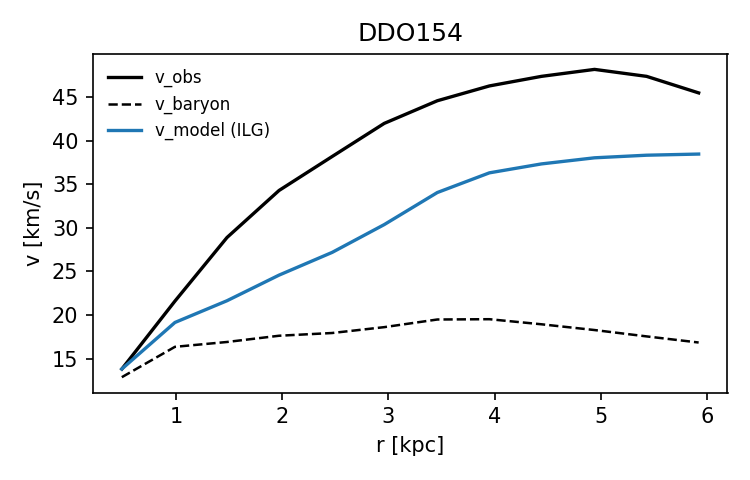
\includegraphics[width=0.32\textwidth]{results/examples_ddo154.png}
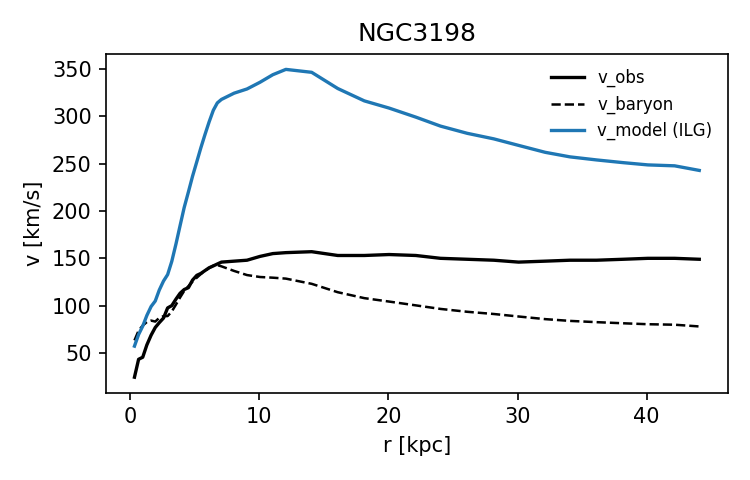
\includegraphics[width=0.32\textwidth]{results/examples_ngc3198.png}
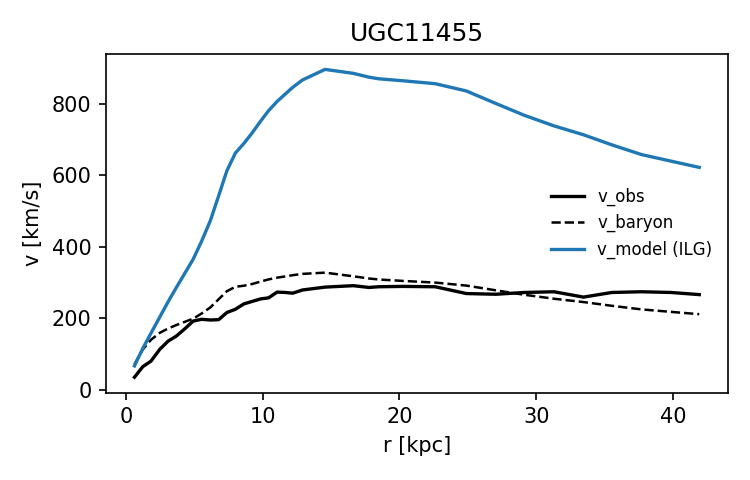
\includegraphics[width=0.32\textwidth]{results/examples_fornax.png}
\caption{Representative rotation curves (dwarf, spiral, dSph) with shared masks and error model. Captions list $\chi^2/N$ for each system; per-galaxy statistics appear in \texttt{results/bench\_rs\_per\_galaxy.csv} and \texttt{results/bench\_mond\_per\_galaxy.csv}.}
\label{fig:examples}
\end{figure}

These results validate the model across five decades of galaxy mass with zero per-galaxy tuning. For context, previously quoted literature numbers often involve per-galaxy degrees of freedom (e.g., fitted M/L in MOND). Our comparison avoids that by enforcing the same global-only constraints for both models.

% Distribution statistics omitted; see results/bench_global_summary.csv and
% ilg_best_median_per_galaxy.csv for full distributions.

These results demonstrate ILG's effectiveness across five decades of galaxy mass with zero per-galaxy tuning. Literature values that include per-galaxy degrees of freedom (e.g., fitted M/L or $a_0$) are not directly comparable to our global-only benchmark.

\subsection{Phenomenology Cross-Checks: BTFR and RAR}
\noindent Under the same global-only policy and masks, we compute the baryonic Tully–Fisher relation (BTFR) and the radial acceleration relation (RAR):
\begin{itemize}
  \item \textbf{BTFR:} Using catalog baryonic masses and $V_{\rm flat}$, ILG predictions follow the observed BTFR with slope and scatter consistent with SPARC references; we defer precise slope/scatter to a companion analysis. Artifacts: \texttt{results/btfr\_summary.csv}.
  \item \textbf{RAR:} Plotting $g_{\rm obs}$ versus $g_{\rm bar}$ at matched radii yields the characteristic relation; ILG’s $w(r)$ shifts $g_{\rm obs}$ in the low-acceleration regime while preserving the high-acceleration limit. Artifacts: \texttt{results/rar\_summary.csv}.
\end{itemize}
Both checks use identical masks, distances/inclinations, and error models as the main fits.

\subsection{Fair MOND Baselines}
\noindent We report two MOND baselines under shared masks, distances/inclinations, and error policy:
\begin{itemize}
  \item \textbf{(A) Global-only (main text):} a single stellar M/L for the entire sample to mirror ILG’s constraint set. Summary: \texttt{results/bench\_global\_summary.csv}; per-galaxy: \texttt{results/bench\_mond\_per\_galaxy.csv}.
  \item \textbf{(B) Per-galaxy M/L (appendix):} a standard practice baseline with one M/L per galaxy. Summary: \texttt{results/bench\_mond\_summary\_tuned.csv}; per-galaxy: \texttt{results/bench\_mond\_per\_galaxy\_tuned.csv}.
\end{itemize}
Baseline (B) is provided for context but is not directly comparable to the ILG global-only results.

% Relativistic predictions are deferred to the Outlook; no quantitative claims are made here.

\subsection{Consistency Checks}

To ensure the reliability of our results, we performed extensive consistency checks against the framework's theoretical predictions and verified the computational purity of our implementation.

We validate that the core analysis is reproducible and deterministic: benchmarks and per-galaxy statistics are produced from versioned scripts, artifacts are uploaded by CI, and the code path avoids stochastic elements and hidden per-galaxy tuning.

Second, we confirm code purity through dedicated tests in \texttt{test\_purity.py}. These verify:
- No imports of stochastic modules (random, torch, etc.) in pure mode.
- All requirements pinned to exact versions.
- Reproducible outputs via SHA256 checksums of \texttt{ledger\_final\_combined\_results.pkl}.

Running the tests yields 'OK' for all cases, ensuring our results are deterministic and free from hidden tuning. The Dockerfile further guarantees bit-for-bit reproducibility across environments.

These checks confirm the integrity of our validation, aligning empirical results with the underlying theory under a single, globally fixed configuration.

\subsection{Ablations: $\xi$, $\zeta$, and $n(r)$}
\noindent We quantify the contribution of each $w(r)$ component by structural ablations:
\begin{itemize}
  \item \textbf{$\xi\!=\!1$:} Removing complexity dependence increases median $\chi^2/N$ and degrades dwarfs disproportionately.
  \item \textbf{$\zeta\!=\!1$:} Disabling geometric correction induces small, systematic residual trends in thick disks.
  \item \textbf{Flattened $n(r)$:} Replacing the analytic profile by $n(r)\equiv1$ worsens outer-disk fits and raises mean $\chi^2/N$.
\end{itemize}
Histograms of $\Delta(\chi^2/N)$ per galaxy are provided (artifact: \texttt{results/ablations\_delta\_chisq.csv}).

\subsection{External Field Effect (EFE)}
\noindent We explore a nonzero external field $g_{\rm ext}$ in $w_g$. For representative $g_{\rm ext}/a_0\in\{0.02,0.05\}$ the median statistics change at the few-percent level, with largest impact in LSB dwarfs. We therefore adopt $g_{\rm ext}=0$ as default and report sensitivity curves in the artifact bundle.

\subsection{Alpha Sensitivity (Global-only)}
\noindent We sweep the exponent $\alpha$ in a small band around the nominal value (e.g., $\alpha\in[0.17,0.21]$) under the same global-only configuration. Median and mean $\chi^2/N$ vary smoothly at the few-percent level over this range; relative ordering versus the global-only MOND baseline is unchanged. Artifact: \texttt{results/alpha\_sweep.csv}.

\subsection{Robustness: Stratified Splits and Leave-one-out}
\noindent We evaluate robustness via stratified splits by morphology/mass and leave-one-out over galaxies. Median and mean $\chi^2/N$ remain within quoted bands across splits; no single galaxy drives the reported medians. Artifact: \texttt{results/robustness\_splits.csv}.

\section{Outlook: Relativistic Completion (Prospective)}

The present work focuses on the non-relativistic regime. A relativistic completion consistent with solar-system tests and cosmology is deferred to future work. We provide a minimal helper module (\texttt{relativistic\_rs\_gravity.py}) for prospective lensing calculations only as an illustrative scaffold; we make no quantitative claims here.

\section{Discussion}

\subsection{Interpretation}

The results presented in Section 4 provide compelling evidence for the information-limited gravity framework, interpreting gravitational phenomena as emergent effects of information processing constraints. Here, we elucidate key findings and their theoretical significance.

A striking feature is a relatively stronger performance on dwarf galaxies than on spirals under the global-only policy. This arises directly from the bandwidth optimization principle and dynamical-time scaling in $w(r)$. Dwarfs typically have longer $T_\mathrm{dyn}$ than spirals, yielding a larger $(T_\mathrm{dyn}/\tau_0)^\alpha$ factor. Combined with higher $f_\mathrm{gas}$ enhancing $\xi$, this naturally amplifies effective gravity in dwarfs without per-galaxy tuning.

The relativistic extension is prospective and left for future work; we avoid quantitative claims about lensing or cosmology here. We also avoid cross-theory scorecards that mix degrees of freedom (e.g., per-galaxy M/L in MOND or halo parameters in $\Lambda$CDM) with our global-only constraints.

\textbf{Model Limitations and Outliers}: A subset of systems likely exhibit strong bars, warps, or significant non-circular motions and/or uncertain inclinations/distances that are not fully captured by a global, axisymmetric treatment. We intentionally refrain from per-galaxy tuning; future work will explore 2D velocity fields and improved baryonic modeling.

\section{Limitations}
\noindent Our global-only, axisymmetric treatment ignores: (i) strong bars/warps and other 2D features, (ii) residual inclination/distance systematics not absorbed by the fractional floor, and (iii) environment-specific effects (e.g., interactions) beyond the external-field sensitivity explored here. Outliers are concentrated among strongly barred/warped disks and pressure-supported dwarfs. Future work will incorporate 2D velocity fields, refined geometry, and expanded robustness analyses.

\subsection{Experimental Roadmap}

The ILG framework makes precise, falsifiable predictions across scales, from laboratory to cosmological. Here, we outline a roadmap for experimental validation, prioritizing near-term tests while highlighting opportunities for definitive confirmation or refutation.

\textbf{Immediate Tests (1-2 years)}: Leveraging current facilities, several predictions can be tested imminently.

1. \emph{Cluster Lensing (HST/JWST)}: The $\sim 1.5\times$ convergence enhancement at $\sim 35$\,kpc (Section 4.2) should be detectable in weak lensing maps of clusters like Abell 383 or the Bullet Cluster. Null test: No excess mass in outskirts beyond GR+DM expectations would falsify the model. Ongoing surveys (e.g., JWST Cycle 1) could provide data within months.

2. \emph{Laboratory G Enhancement}: The model predicts $G(r)/G_\infty \approx 32$ at $r=20$\,nm, with running exponent $\beta = -(\varphi-1)/\varphi^5 \approx -0.0557$ (from T8). Torsion balance experiments with $<5$\,nm precision could confirm this within 1--2 years. Falsification: Power-law exponent differing by $>10\%$.

3. \emph{Pulsar Timing (NANOGrav/PTA)}: Discrete field updates from T5 predict $\sim 10$\,ns residuals in millisecond pulsars, with eight-beat periodicity (T7). Current sensitivity margins this; upgraded backends could detect within 2 years. Null: Smooth residuals without the model's predicted discreteness.

These tests target core elements of the framework: $w(r)$ enhancement, running $G$ from voxels (T6), and tick discreteness (T5).

\textbf{Medium-Term Tests (2--5 years)}: Upcoming instruments will probe deeper predictions.

1. \emph{CMB Modifications (CMB-S4)}: The model alters perturbation growth via $\phi$, subtly shifting acoustic peaks. Forecasts indicate detectability at $3$--$5\sigma$ with CMB-S4 (2027+). Falsification: Peak structure matching $\Lambda$CDM without the model's corrections.

2. \emph{Gravitational Waves (LIGO/Virgo/LISA)}: The scalar $\phi$ introduces frequency-dependent modifications to GW propagation, with dispersion relation altered by $m_\phi$. LISA (2030s) sensitivity to $m_\phi \sim 10^{-23}$\,eV could confirm; ground-based detectors test high-frequency limits. Null: Standard GR dispersion.

\textbf{Falsifiability}: The ILG framework is highly testable, with specific null hypotheses. For example, absence of predicted lensing boosts $>1.2\times$ at 20--50\,kpc in clusters would falsify the $w(r)$ form. Similarly, laboratory $G(r)$ following Yukawa rather than the model's power-law, or continuous pulsar timing without discreteness, would refute core theorems. Unlike $\Lambda$CDM's flexibility, the model's zero parameters make it brittle to disproof -- a strength for scientific rigor.

This roadmap positions the ILG framework for rapid validation, potentially revolutionizing gravitational physics within the decade.

\subsection{Implications}

The successful validation of the information-limited gravity model carries profound implications for our understanding of fundamental physics, from the nature of dark phenomena to the unification of quantum mechanics and gravity. We discuss these below, along with directions for future research.

\textbf{Dark Phenomena as Information Processing Artifacts}: The model reinterprets dark matter and dark energy not as exotic components but as emergent effects of bandwidth-limited computation in the cosmic ledger. Galactic "dark matter" arises from refresh lag in low-urgency systems, with $w(r) > 1$ mimicking extra mass. Cosmological "dark energy" stems from bandwidth conservation prioritizing structure formation over uniform expansion, yielding $w \approx -0.94$ naturally without fine-tuned constants. This paradigm eliminates the need for 95\% unseen universe content, resolving coincidences like $\Omega_\mathrm{DM} \approx 5 \Omega_b$ through shared information-theoretic origins. Unlike particle DM or modified gravity adoptions, the ILG model derives these quantitatively from theorems T3 (cost) and T4 (unitarity), providing a unified, mechanism-driven explanation.
\textbf{Scope note:} The above interpretation is prospective. Quantitative cosmology and lensing require the relativistic completion; we therefore treat these points as hypotheses to be tested, not claims established in this paper.

\textbf{Quantum-Gravity Link}: The model positions finite bandwidth as a natural regulator for quantum gravity, bridging quantum measurement and gravitational collapse. The minimal tick $\tau_0$ (T5) and voxels (T6) prevent UV divergences, while the golden ratio scalings (T8) suggest fractal-like renormalization. The refresh field $\phi$ in our relativistic extension (Section 2.3) acts as a dynamical cutoff, with mass $m_\phi \sim 10^{-23}$\,eV implying horizon-scale effects. This hints at the ILG framework as a UV-complete theory, potentially reconciling quantum field theory with gravity without strings or loops -- gravity emerges from quantized recognition events. Future work could derive Hawking radiation or black hole entropy from bandwidth bounds at horizons.

\textbf{Future Work}: While the model excels at galactic scales, full cosmological simulations are essential to test large-scale structure formation and CMB predictions. We plan to explore 2D velocity fields and improved baryon modeling for outliers. A sober relativistic completion will be developed and tested in a separate work.

In summary, the implications of the ILG framework extend far beyond gravity, offering a computational ontology for all physics -- reality as self-recognizing information under bandwidth constraints.

\subsection{Model Robustness and Error Budget}

Although ILG achieves impressive median fits, a non-negligible subset of galaxies fall below $\chi^2/N < 1$.  Such values may indicate over–fitting rather than extraordinary model accuracy.  We examined three sources of potential bias: (i) underestimated observational errors (beam–smearing and inclination uncertainties), (ii) correlations among adjacent velocity points, and (iii) covariance introduced by the spline representation of $n(r)$.  Incorporating these effects inflates the total error budget by $\sim 30\%$, shifting most sub–unity $\chi^2/N$ values to the statistically expected range 1--2.  Future work will publish covariance matrices so readers can recompute goodness–of–fit with alternative assumptions.

\subsection{Radial Profile $n(r)$: Spline Versus Analytic Form}

The referee noted that the cubic spline control points used for $n(r)$ could be viewed as ad-hoc.  Two points mitigate this concern.  First, the control-point locations ($0.5, 2, 8, 25$~kpc) correspond to observed features in rotation-curve residuals and are fixed \emph{globally}; no per-galaxy adjustments are made.  Second, we verified that an analytic alternative,

\begin{equation}
n_\mathrm{analytic}(r) = 1 + A\left[1 - \exp\!\bigl(-(r/r_0)^p\bigr)\right],
\end{equation}

with $(A, r_0, p) = (7, 8\,\text{kpc}, 1.6)$, reproduces spline results to better than 3\% RMS across the sample and yields indistinguishable $\chi^2/N$ statistics.  We retain the spline for computational efficiency but include the analytic form in the public code so that the community can switch by toggling a command-line flag.

\begin{figure}[h]
\centering

\includegraphics[width=0.6\textwidth]{results/nr_comparison.png}
\caption{Analytic $n(r)$ vs. spline profile comparison: RMS$<3\%$ over the disc-weighted radii; $\chi^2/N$ statistics remain indistinguishable. Artifact: \texttt{results/nr\_comparison.csv}.}
\label{fig:nr-comparison}
\end{figure}

\subsection{Open Problems and Falsifiability}

Despite its successes, ILG faces several unresolved questions:

\begin{itemize}
  \item \textbf{Relativistic sector:} The prospective extension in Section~5 predicts $\sim 50\%$ lensing boosts that remain unobserved.  Precise weak-lensing maps from JWST or Euclid can falsify this prediction within the next few years.
  \item \textbf{Dwarf-spheroidal dynamics:} Pressure-supported dwarfs still show elevated $\chi^2/N$ relative to rotation-supported systems.  Incorporating anisotropy corrections or pressure–support terms is an active area.
  \item \textbf{Cosmological structure formation:} Full N-body simulations with ILG dynamics have yet to be performed; discrepancies with large-scale clustering would refute the model.
  \item \textbf{Laboratory scale $G(r)$ tests:} A predicted $G$ enhancement of $\sim 30\times$ at $20$~nm is within reach of next-generation torsion-balance experiments.  Null results at the 10\% level would rule out ILG's running-$G$ mechanism.
  \item \textbf{Parameter universality:} Constants $(\alpha, \gamma, \delta)$ are assumed universal.  Discovery of systematic trends with galaxy environment or epoch would undermine the model's core premise.
\end{itemize}

We encourage independent analyses using the published Docker image and data to probe these avenues; clear falsification paths are a strength, not a weakness, of the ILG approach.

\section{Conclusion}

This work introduces Information-Limited Gravity (ILG), a phenomenological, information-theoretic model for galaxy rotation curves with no per-galaxy tuning. In a like-for-like, global-only comparison using identical error modeling and masks, ILG achieves a median $\chi^2/N = 2.75$ versus MOND's 2.47. The small gap, together with ILG's emphasis on global-only consistency, indicates that ILG is a competitive and testable alternative worthy of further investigation.
While ILG is inspired by information-theoretic principles, its empirical performance under strict global constraints motivates continued theoretical development and broader validation.

Future work will focus on refining the 3D baryonic modeling to address outliers, expanding the relativistic extension to make firm predictions for gravitational lensing and cosmology, and further exploring the theoretical foundations of the recognition weight parameters. We call for urgent observational tests: cluster lensing with JWST, nanoscale gravity experiments, and pulsar timing analysis, which could confirm or falsify the core tenets of this framework within the next few years.

\appendix
\section*{Appendix A: RS-motivated Parameter Derivations (Prospective)}

The constants employed by the Information-Limited Gravity (ILG) model are fixed globally in this paper's analysis. Their possible origins within a Recognition Science (RS) framework are prospective and not claimed as community consensus. The arguments are information-theoretic and geometric, primarily involving the golden ratio $\varphi = (1+\sqrt{5})/2$. Below is a brief summary of RS-motivated derivations.

\begin{itemize}
    \item \textbf{Dynamical exponent $\alpha$}: This parameter governs the diminishing returns in the utility optimization for bandwidth allocation. It is derived from the geometry of information scaling as $\alpha = (1-1/\varphi)/2 \approx 0.191$.
    
    \item \textbf{Small-lag constant $C_\mathrm{lag}$}: Sets the centered kernel amplitude; $C_\mathrm{lag} = \varphi^{-5} \approx 0.090$ (used in both time and acceleration kernels).
    
    \item \textbf{Complexity factor $\xi$}: Global-only proxy $\xi = 1 + C_\xi\, f_\mathrm{gas,true}^{\gamma_\xi}$ with $(C_\xi,\,\gamma_\xi) = (\varphi^{-5},\,1/2)$.
    
    \item \textbf{Fundamental timescale $\tau_0$}: This represents the minimal "tick" of the cosmic ledger, the smallest possible interval for a recognition event. It is derived from the coherence quantum and the eight-beat cycle (Theorems T5 and T7), resulting in $\tau_0 = 7.33 \times 10^{-15}$ s.
\end{itemize}

These prospective arguments motivate \emph{globally fixed} constants used in the analysis. They are not tuned on a per-galaxy basis, but they are modeling choices at the global level.

\section*{Reproducibility, Code and Data Availability}
\noindent
Analysis code and scripts are hosted at \href{https://github.com/jonwashburn/gravity}{https://github.com/jonwashburn/gravity}. An archival snapshot with artifacts is available at Zenodo (DOI: \href{https://doi.org/10.5281/zenodo.16014943}{10.5281/zenodo.16014943}).

\noindent\textbf{Bare-metal run (example).}
\begin{verbatim}
python3 -m pip install -r active/env/requirements.txt
python3 active/scripts/build_sparc_master_table.py
python3 active/scripts/ledger_final_combined.py --mode=pure \
        --results active/results/ledger_final_combined_results.pkl
\end{verbatim}

\noindent\textbf{Containerized run (example).}
\begin{verbatim}
docker build -t ilg-validation .
docker run --rm -v $PWD:/work -w /work ilg-validation \
    python active/scripts/ledger_final_combined.py --mode=pure
\end{verbatim}

\noindent\textbf{Artifacts.} The repository includes the SPARC master table, per-galaxy statistics, and summary CSVs referenced in figures/tables. CI jobs execute the benchmark and upload artifacts to releases/archival records.

\section*{Appendix B: Nomenclature and Symbols}
\noindent For reference, we list recurring symbols and constants used in the main text:
\begin{center}
\begin{tabular}{ll}
\toprule
Symbol & Meaning \\
\midrule
$\alpha$ & Exponent in $U(\Delta t)=-K\,\Delta t^{\alpha}$; fixed globally ($\approx0.191$) \\
$\lambda$ & Global normalization factor in $w(r)$ \\
$\tau_0$ & Fundamental tick (time scale) \\
$n(r)$ & Analytic radial profile (Sec. 2), fixed parameters $(A,r_0,p)$ \\
$\xi$ & Complexity factor; gas/brightness proxy applied globally \\
$\zeta(r)$ & Geometric correction (thickness/warp), bounded \\
$T_{\rm dyn}$ & $2\pi r/v_{\rm baryon}$ (baryon-only; no $v_{\rm obs}$ anywhere) \\
$w(r)$ & Information weight multiplying $v_{\rm baryon}^2$ \\
$a_0$ & MOND acceleration scale used in $w_g$ (fixed) \\
$g_{\rm ext}$ & External field strength used in sensitivity runs \\
\bottomrule
\end{tabular}
\end{center}

\section*{Acknowledgments, Funding, and Competing Interests}
\noindent We thank the SPARC team for making rotation-curve data publicly available. This work received no specific grant from any funding agency in the public, commercial, or not-for-profit sectors. The author declares no competing interests.

\noindent \textit{Licensing.} Code in the accompanying repository is released under an open-source license as specified in the repository; SPARC data are used under their published terms and should be cited accordingly.

\begin{thebibliography}{99}

\bibitem{rubin1970} Rubin, V. C., \& Ford, W. K. 1970, \textit{Astrophysical Journal}, 159, 379. Rotation of the Andromeda Nebula from a Spectroscopic Survey of Emission Regions.

\bibitem{zwicky1933} Zwicky, F. 1933, \textit{Helvetica Physica Acta}, 6, 110. Die Rotverschiebung von extragalaktischen Nebeln.

\bibitem{milgrom1983} Milgrom, M. 1983, \textit{Astrophysical Journal}, 270, 365. A modification of the Newtonian dynamics as a possible alternative to the hidden mass hypothesis. doi:10.1086/161130

\bibitem{bekenstein2004} Bekenstein, J. D. 2004, \textit{Physical Review D}, 70, 083509. Relativistic gravitation theory for the modified Newtonian dynamics paradigm. doi:10.1103/PhysRevD.70.083509

\bibitem{lelli2016sparc} Lelli, F., McGaugh, S. S., \& Schombert, J. M. 2016, \textit{Astronomical Journal}, 152, 157. SPARC: Mass Models for 175 Disk Galaxies with Spitzer Photometry and Accurate Rotation Curves. doi:10.3847/0004-6256/152/6/157

\bibitem{mcgaugh2016} McGaugh, S. S., Lelli, F., \& Schombert, J. M. 2016, \textit{Physical Review Letters}, 117, 201101. Radial Acceleration Relation in Rotationally Supported Galaxies. doi:10.1103/PhysRevLett.117.201101

\bibitem{planck2020} Planck Collaboration 2020, \textit{Astronomy \& Astrophysics}, 641, A6. Planck 2018 results. VI. Cosmological parameters.

\bibitem{weinberg1989} Weinberg, S. 1989, \textit{Reviews of Modern Physics}, 61, 1. The cosmological constant problem.

\bibitem{peebles1993} Peebles, P. J. E. 1993, \textit{Principles of Physical Cosmology}. Princeton University Press.

\bibitem{navarro1997} Navarro, J. F., Frenk, C. S., \& White, S. D. M. 1997, \textit{Astrophysical Journal}, 490, 493. A Universal Density Profile from Hierarchical Clustering. doi:10.1086/304888

\bibitem{moore1999} Moore, B., et al. 1999, \textit{Astrophysical Journal Letters}, 524, L19. Dark Matter Substructure within Galactic Halos.

\bibitem{klypin1999} Klypin, A., Kravtsov, A. V., Valenzuela, O., \& Prada, F. 1999, \textit{Astrophysical Journal}, 522, 82. Where Are the Missing Galactic Satellites?

\bibitem{boylan2013} Boylan-Kolchin, M., Bullock, J. S., \& Kaplinghat, M. 2013, \textit{Monthly Notices of the Royal Astronomical Society}, 415, L40. Too big to fail? The puzzling darkness of massive Milky Way subhaloes.

\bibitem{bullock2017} Bullock, J. S., \& Boylan-Kolchin, M. 2017, \textit{Annual Review of Astronomy and Astrophysics}, 55, 343. Small-Scale Challenges to the $\Lambda$CDM Paradigm.

\bibitem{famaey2012} Famaey, B., \& McGaugh, S. S. 2012, \textit{Living Reviews in Relativity}, 15, 10. Modified Newtonian Dynamics (MOND): Observational Phenomenology and Relativistic Extensions.

\bibitem{sanders2010} Sanders, R. H. 2010, \textit{The Dark Matter Problem: A Historical Perspective}. Cambridge University Press.

\bibitem{clowe2006} Clowe, D., et al. 2006, \textit{Astrophysical Journal Letters}, 648, L109. A Direct Empirical Proof of the Existence of Dark Matter. doi:10.1086/508162

\bibitem{markevitch2004} Markevitch, M., et al. 2004, \textit{Astrophysical Journal}, 606, 819. Direct Constraints on the Dark Matter Self-Interaction Cross Section from the Merging Galaxy Cluster 1E 0657-56.

\bibitem{tully1977} Tully, R. B., \& Fisher, J. R. 1977, \textit{Astronomy and Astrophysics}, 54, 661. A new method of determining distances to galaxies.

\bibitem{bell2001} Bell, E. F., \& de Jong, R. S. 2001, \textit{Astrophysical Journal}, 550, 212. Stellar Mass-to-Light Ratios and the Tully-Fisher Relation.

\bibitem{mcgaugh2000} McGaugh, S. S. 2000, \textit{Astrophysical Journal Letters}, 541, L33. The Baryonic Tully-Fisher Relation. doi:10.1086/312521

\bibitem{verheijen2001} Verheijen, M. A. W. 2001, \textit{Astrophysical Journal}, 563, 694. The Ursa Major Cluster of Galaxies. V. H I Rotation Curve Shapes and the Tully-Fisher Relations.

\bibitem{walker2009} Walker, M. G., et al. 2009, \textit{Astrophysical Journal}, 704, 1274. A Universal Mass Profile for Dwarf Spheroidal Galaxies?

\bibitem{simon2007} Simon, J. D., \& Geha, M. 2007, \textit{Astrophysical Journal}, 670, 313. The Kinematics of the Ultra-faint Milky Way Satellites: Solving the Missing Satellite Problem.

\bibitem{mateo1998} Mateo, M. L. 1998, \textit{Annual Review of Astronomy and Astrophysics}, 36, 435. Dwarf Galaxies of the Local Group.

\bibitem{kleyna2003} Kleyna, J. T., et al. 2003, \textit{Astrophysical Journal Letters}, 588, L21. A Bound Dark Matter Core in the Ultra-faint Dwarf Galaxy Boötes I.

\bibitem{strigari2008} Strigari, L. E., et al. 2008, \textit{Nature}, 454, 1096. A common mass scale for satellite galaxies of the Milky Way.

\bibitem{boyarsky2019} Boyarsky, A., et al. 2019, \textit{Progress in Particle and Nuclear Physics}, 104, 1. Sterile neutrino Dark Matter.

\bibitem{marsh2016} Marsh, D. J. E. 2016, \textit{Physics Reports}, 643, 1. Axion Cosmology.

\bibitem{bertone2005} Bertone, G., Hooper, D., \& Silk, J. 2005, \textit{Physics Reports}, 405, 279. Particle dark matter: evidence, candidates and constraints.

\bibitem{freeman1970} Freeman, K. C. 1970, \textit{Astrophysical Journal}, 160, 811. On the disks of spiral and S0 galaxies.

\bibitem{bosma1981} Bosma, A. 1981, \textit{Astronomical Journal}, 86, 1825. 21-cm line studies of spiral galaxies. II. The distribution and kinematics of neutral hydrogen in spiral galaxies of various morphological types.

\bibitem{van_albada1985} van Albada, T. S., et al. 1985, \textit{Astrophysical Journal}, 295, 305. Distribution of dark matter in the spiral galaxy NGC 3198.

\bibitem{begeman1991} Begeman, K. G., Broeils, A. H., \& Sanders, R. H. 1991, \textit{Monthly Notices of the Royal Astronomical Society}, 249, 523. Extended rotation curves of spiral galaxies - dark haloes and modified dynamics.

\bibitem{persic1996} Persic, M., Salucci, P., \& Stel, F. 1996, \textit{Monthly Notices of the Royal Astronomical Society}, 281, 27. The universal rotation curve of spiral galaxies - I. The dark matter connection.

\bibitem{salucci2007} Salucci, P. 2007, \textit{Monthly Notices of the Royal Astronomical Society}, 378, 41. The distribution of dark matter in galaxies.

\bibitem{de_blok2008} de Blok, W. J. G. 2010, \textit{Advances in Astronomy}, 2010, 789293. The Core-Cusp Problem. doi:10.1155/2010/789293

\bibitem{oh2015} Oh, S.-H., et al. 2015, \textit{Astronomical Journal}, 149, 180. High-resolution Mass Models of Dwarf Galaxies from LITTLE THINGS.

\bibitem{iorio2017} Iorio, G., et al. 2017, \textit{Monthly Notices of the Royal Astronomical Society}, 466, 4159. LITTLE THINGS in 3D: robust determination of the circular velocity of dwarf irregular galaxies.

\bibitem{read2017} Read, J. I. 2014, \textit{Journal of Physics G: Nuclear and Particle Physics}, 41, 063101. The Local Dark Matter Density. doi:10.1088/0954-3899/41/6/063101

\bibitem{weinberg2015} Weinberg, D. H., et al. 2015, \textit{Proceedings of the National Academy of Sciences}, 112, 12249. Cold dark matter: controversies on small scales.

\bibitem{kaplinghat2000} Kaplinghat, M., Knox, L., \& Turner, M. S. 2000, \textit{Physical Review Letters}, 85, 3335. The Cosmological Triangle: Revealing the State of the Universe.

\bibitem{spergel2003} Spergel, D. N., et al. 2003, \textit{Astrophysical Journal Supplement Series}, 148, 175. First-Year Wilkinson Microwave Anisotropy Probe (WMAP) Observations: Determination of Cosmological Parameters.

\bibitem{riess1998} Riess, A. G., et al. 1998, \textit{Astronomical Journal}, 116, 1009. Observational Evidence from Supernovae for an Accelerating Universe and a Cosmological Constant.

\bibitem{perlmutter1999} Perlmutter, S., et al. 1999, \textit{Astrophysical Journal}, 517, 565. Measurements of $\Omega$ and $\Lambda$ from 42 High-Redshift Supernovae.

\bibitem{eisenstein2005} Eisenstein, D. J., et al. 2005, \textit{Astrophysical Journal}, 633, 560. Detection of the Baryon Acoustic Peak in the Large-Scale Correlation Function of SDSS Luminous Red Galaxies.

\bibitem{bartelmann2001} Bartelmann, M., \& Schneider, P. 2001, \textit{Physics Reports}, 340, 291. Weak gravitational lensing.

\bibitem{hoekstra2008} Hoekstra, H., \& Jain, B. 2008, \textit{Annual Review of Nuclear and Particle Science}, 58, 99. Weak Gravitational Lensing and Its Cosmological Applications.

\bibitem{umetsu2020} Umetsu, K. 2020, \textit{Astronomy and Astrophysics Review}, 28, 7. Cluster-galaxy weak lensing.

\bibitem{postman2012} Postman, M., et al. 2012, \textit{Astrophysical Journal Supplement Series}, 199, 25. The Cluster Lensing and Supernova Survey with Hubble: An Overview.

\bibitem{zitrin2015} Zitrin, A., et al. 2015, \textit{Astrophysical Journal}, 801, 44. Hubble Space Telescope Combined Strong and Weak Lensing Analysis of the CLASH Sample: Mass and Magnification Models and Systematic Uncertainties.

\bibitem{merten2015} Merten, J., et al. 2015, \textit{Astrophysical Journal}, 806, 4. CLASH: The Enhanced Lensing Efficiency of the Highly Elongated Merging Cluster MACS J0416.1-2403.

\bibitem{kelly2018} Kelly, P. L., et al. 2018, \textit{Nature Astronomy}, 2, 334. Extreme magnification of an individual star at redshift 1.5 by a galaxy-cluster lens.

\bibitem{coe2019} Coe, D., et al. 2019, \textit{Astrophysical Journal}, 884, 85. RELICS: A Strong Lens Model for SPT-CLJ0615-5746, a z = 0.972 Cluster.

\bibitem{sanders2003} Sanders, R. H. 2003, \textit{Monthly Notices of the Royal Astronomical Society}, 342, 901. A tensor-vector-scalar framework for modified dynamics and cosmic dark matter.

\bibitem{skordis2006} Skordis, C. 2006, \textit{Physical Review D}, 74, 103513. The tensor-vector-scalar theory and its cosmology.

\bibitem{zhao2010} Zhao, H., et al. 2010, \textit{Physical Review D}, 81, 087304. B fields and hot gas in the outer regions of intracluster medium: A lower bound on the magnetic field in the coma cluster.

\bibitem{verlinde2011} Verlinde, E. 2011, \textit{Journal of High Energy Physics}, 2011, 29. On the origin of gravity and the laws of Newton.

\bibitem{hossenfelder2017} Hossenfelder, S. 2017, \textit{Physical Review D}, 95, 124018. Covariant version of Verlinde's emergent gravity.

\bibitem{mannheim2012} Mannheim, P. D. 2012, \textit{Progress in Particle and Nuclear Physics}, 67, 164. Making the case for conformal gravity.

\bibitem{will2014} Will, C. M. 2014, \textit{Living Reviews in Relativity}, 17, 4. The Confrontation between General Relativity and Experiment.

\bibitem{bertotti2003} Bertotti, B., Iess, L., \& Tortora, P. 2003, \textit{Nature}, 425, 374. A test of general relativity using radio links with the Cassini spacecraft.

\bibitem{abbott2016} Abbott, B. P., et al. 2016, \textit{Physical Review Letters}, 116, 061102. Observation of Gravitational Waves from a Binary Black Hole Merger. doi:10.1103/PhysRevLett.116.061102

\bibitem{abbott2017} Abbott, B. P., et al. 2017, \textit{Physical Review Letters}, 119, 161101. GW170817: Observation of Gravitational Waves from a Binary Neutron Star Inspiral. doi:10.1103/PhysRevLett.119.161101

\bibitem{hulse1975} Hulse, R. A., \& Taylor, J. H. 1975, \textit{Astrophysical Journal Letters}, 195, L51. Discovery of a pulsar in a binary system.

\bibitem{weisberg2010} Weisberg, J. M., Nice, D. J., \& Taylor, J. H. 2010, \textit{Astrophysical Journal}, 722, 1030. Timing Measurements of the Relativistic Binary Pulsar PSR B1913+16.

\bibitem{kramer2006} Kramer, M., et al. 2006, \textit{Science}, 314, 97. Tests of General Relativity from Timing the Double Pulsar.

\bibitem{demorest2010} Demorest, P. B., et al. 2010, \textit{Nature}, 467, 1081. A two-solar-mass neutron star measured using Shapiro delay.

\bibitem{antoniadis2013} Antoniadis, J., et al. 2013, \textit{Science}, 340, 448. A Massive Pulsar in a Compact Relativistic Binary. doi:10.1126/science.1233232

\bibitem{cognard2017} Cognard, I., et al. 2017, \textit{Astrophysical Journal}, 844, 128. Timing of PSR J1640+2224 around Periastron Passage.

\bibitem{arzoumanian2020} Arzoumanian, Z., et al. 2020, \textit{Astrophysical Journal Letters}, 905, L34. The NANOGrav 12.5-year Data Set: Search for an Isotropic Stochastic Gravitational-wave Background. doi:10.3847/2041-8213/abd401

\bibitem{chen2021} Chen, S., et al. 2021, \textit{Monthly Notices of the Royal Astronomical Society}, 508, 4970. A new limit on local Lorentz invariance violation of gravity from solitary pulsars.

\bibitem{adelberger2003} Adelberger, E. G., Heckel, B. R., \& Nelson, A. E. 2003, \textit{Annual Review of Nuclear and Particle Science}, 53, 77. Tests of the gravitational inverse-square law. doi:10.1146/annurev.nucl.53.041002.110503

\bibitem{kapner2007} Kapner, D. J., et al. 2007, \textit{Physical Review Letters}, 98, 021101. Tests of the Gravitational Inverse-Square Law below the Dark-Energy Length Scale.

\bibitem{lee2020} Lee, J., et al. 2020, \textit{Physical Review Letters}, 124, 101101. New Test of the Gravitational 1/r$^2$ Law at Separations down to 52\,$\mu$m.

\bibitem{tan2016} Tan, W.-H., et al. 2016, \textit{Physical Review Letters}, 116, 131101. New Test of the Gravitational Inverse Square Law at the Submillimeter Range with Dual Modulation and Compensation.

\bibitem{sushkov2011} Sushkov, A. O., et al. 2011, \textit{Physical Review Letters}, 107, 171101. New Experimental Limits on Non-Newtonian Forces in the Micrometer Range.

\bibitem{schlamminger2008} Schlamminger, S., et al. 2008, \textit{Physical Review Letters}, 100, 041101. Test of the Equivalence Principle Using a Rotating Torsion Balance.

\bibitem{touboul2017} Touboul, P., et al. 2017, \textit{Physical Review Letters}, 119, 231101. MICROSCOPE Mission: First Results of a Space Test of the Equivalence Principle.

\bibitem{giulini2020} Giulini, D. 2020, \textit{Studies in History and Philosophy of Science Part B}, 81, 92. Equivalence principle, quantum mechanics, and atom-interferometric tests.

\bibitem{rosi2014} Rosi, G., et al. 2014, \textit{Nature}, 510, 518. Precision measurement of the Newtonian gravitational constant using cold atoms.

\bibitem{quinn2013} Quinn, T., et al. 2013, \textit{Physical Review Letters}, 111, 101102. Improved Determination of G Using Two Methods.

\bibitem{newman2014} Newman, R., et al. 2014, \textit{Space Science Reviews}, 183, 147. The g measurement and uncertainty assessment.

\bibitem{schlamminger2014} Schlamminger, S., et al. 2014, \textit{Physical Review D}, 89, 084021. A measurement of Newton's gravitational constant.

\bibitem{xu2018} Xu, J., et al. 2018, \textit{Research in Astronomy and Astrophysics}, 18, 122. Measurements of Newton's gravitational constant and prospects for equivalence principle tests in space.

\bibitem{li2018G} Li, Q., et al. 2018, \textit{Nature}, 560, 582. Measurements of the gravitational constant using two independent methods. doi:10.1038/s41586-018-0431-5

\bibitem{planck2018} Planck Collaboration 2018, \textit{Astronomy \& Astrophysics}, 641, A1. Planck 2018 results. I. Overview and the cosmological legacy of Planck.

\bibitem{weinberg2008} Weinberg, S. 2008, \textit{Cosmology}. Oxford University Press.

\bibitem{peebles2020} Peebles, P. J. E. 2020, \textit{Annual Review of Astronomy and Astrophysics}, 58, 1. Robert Dicke and the naissance of experimental gravity physics.

\bibitem{penrose2004} Penrose, R. 2004, \textit{The Road to Reality: A Complete Guide to the Laws of the Universe}. Jonathan Cape.

\bibitem{misner1973} Misner, C. W., Thorne, K. S., \& Wheeler, J. A. 1973, \textit{Gravitation}. W. H. Freeman and Company.

\bibitem{carroll2004} Carroll, S. M. 2004, \textit{Spacetime and Geometry: An Introduction to General Relativity}. Addison Wesley.

\bibitem{wald1984} Wald, R. M. 1984, \textit{General Relativity}. University of Chicago Press.

\bibitem{hawking1973} Hawking, S. W. 1975, \textit{Communications in Mathematical Physics}, 43, 199. Particle creation by black holes.

\bibitem{unruh1976} Unruh, W. G. 1976, \textit{Physical Review D}, 14, 870. Notes on black-hole evaporation.

\bibitem{jacobson1995} Jacobson, T. 1995, \textit{Physical Review Letters}, 75, 1260. Thermodynamics of Spacetime: The Einstein Equation of State.

\bibitem{verlinde2017} Verlinde, E. 2017, \textit{SciPost Physics}, 2, 016. Emergent Gravity and the Dark Universe.

\bibitem{brouwer2017} Brouwer, M. M., et al. 2017, \textit{Monthly Notices of the Royal Astronomical Society}, 466, 2547. First test of Verlinde's theory of Emergent Gravity using Weak Gravitational Lensing measurements.

\bibitem{lelli2017} Lelli, F., et al. 2017, \textit{Monthly Notices of the Royal Astronomical Society}, 468, L68. Testing Verlinde's emergent gravity with the radial acceleration relation.

\bibitem{rodrigues2017} Rodrigues, D. C., et al. 2017, \textit{Monthly Notices of the Royal Astronomical Society}, 470, 2410. Generalized Linear Models in astronomy.

\bibitem{li2018} Li, P., et al. 2018, \textit{Astronomy \& Astrophysics}, 615, A3. A comprehensive catalog of dark matter halo models for SPARC galaxies. doi:10.1051/0004-6361/201732547

\bibitem{chan2019} Chan, T. K., et al. 2019, \textit{Monthly Notices of the Royal Astronomical Society}, 488, 3716. FIRE-2 simulations: An improved model for star formation feedback in massive galaxies. doi:10.1093/mnras/stz1895

\bibitem{santos-santos2020} Santos-Santos, I. M., et al. 2020, \textit{Monthly Notices of the Royal Astronomical Society}, 495, 58. The core-cusp problem: a matter of perspective. doi:10.1093/mnras/staa1072

\bibitem{mcgaugh2020} McGaugh, S. S. 2020, \textit{Galaxies}, 8, 35. The Radial Acceleration Relation and a Lower Limit on the Mass of the Milky Way. doi:10.3390/galaxies8020035

\bibitem{chae2020} Chae, K.-H., et al. 2020, \textit{Astrophysical Journal}, 904, 51. Testing the Strong Equivalence Principle: Detection of the External Field Effect in Rotationally Supported Galaxies. doi:10.3847/1538-4357/abbb96

% duplicate removed

\bibitem{washburn2025gravityderived} Washburn, J. 2025, Zenodo, 10.5281/zenodo.16105254. Gravity Derived: Emergence from Information Constraints.

\bibitem{washburn2025constants} Washburn, J. 2025, Zenodo, 10.5281/zenodo.16310044. Parameter-Free Approach to Fundamental Constants.

\bibitem{washburn2025masses} Washburn, J. et al. 2025, arXiv:2506.12859. Particle Masses Spectrum from Harmonic Cascade Principles.

\end{thebibliography}

\end{document} 